\documentclass[10pt, compress]{beamer}

\usetheme[numbering=fraction, sectionpage=none, progressbar=frametitle]{m}
\usepackage{booktabs}
\usepackage{array}
\usepackage{listings}
\usepackage{graphicx}
\usepackage[english]{babel}
\usepackage[scale=2]{ccicons}

\usepackage{pgfplots}
\usepgfplotslibrary{dateplot}

\graphicspath{{./img/}}

\title{Autotuning GPU Compiler Parameters with OpenTuner}
\subtitle{}
\author{\footnotesize Pedro Bruel \\ {\scriptsize phrb@ime.usp.br} \\[0.2cm]
Marcos Amarís \\ {\scriptsize amaris@ime.usp.br} \\[0.2cm]
Alfredo Goldman \\{\scriptsize gold@ime.usp.br} }
\institute{
\includegraphics[height=1.5cm]{imelogo} \\ \enspace
\includegraphics[height=0.5cm]{fapesp-logo}\enspace
\includegraphics[height=0.8cm]{capes-logo}\enspace
\includegraphics[height=0.7cm]{cnpq-logo}\enspace
\includegraphics[height=0.4cm]{nvidia-logo}\enspace
\includegraphics[height=0.5cm]{hp-logo}\\[0.2cm] Instituto de Matemática e Estatística \\ Universidade de São Paulo}
\date{\scriptsize October 19, 2015}

\begin{document}

\maketitle

\begin{frame}[fragile]
  \frametitle{Contribution}
  It is possible to optimize GPU applications for different devices
  by \alert{automatically tuning} compilation parameters.
\end{frame}

\begin{frame}[fragile]
  \frametitle{Autotuning}
  \begin{columns}
      \column{0.5\textwidth}
      \centering
      Configurations and Optimizations
      \column{0.5\textwidth}
      \centering
      Search Space
  \end{columns}
  \begin{figure}[H]
      \centering
      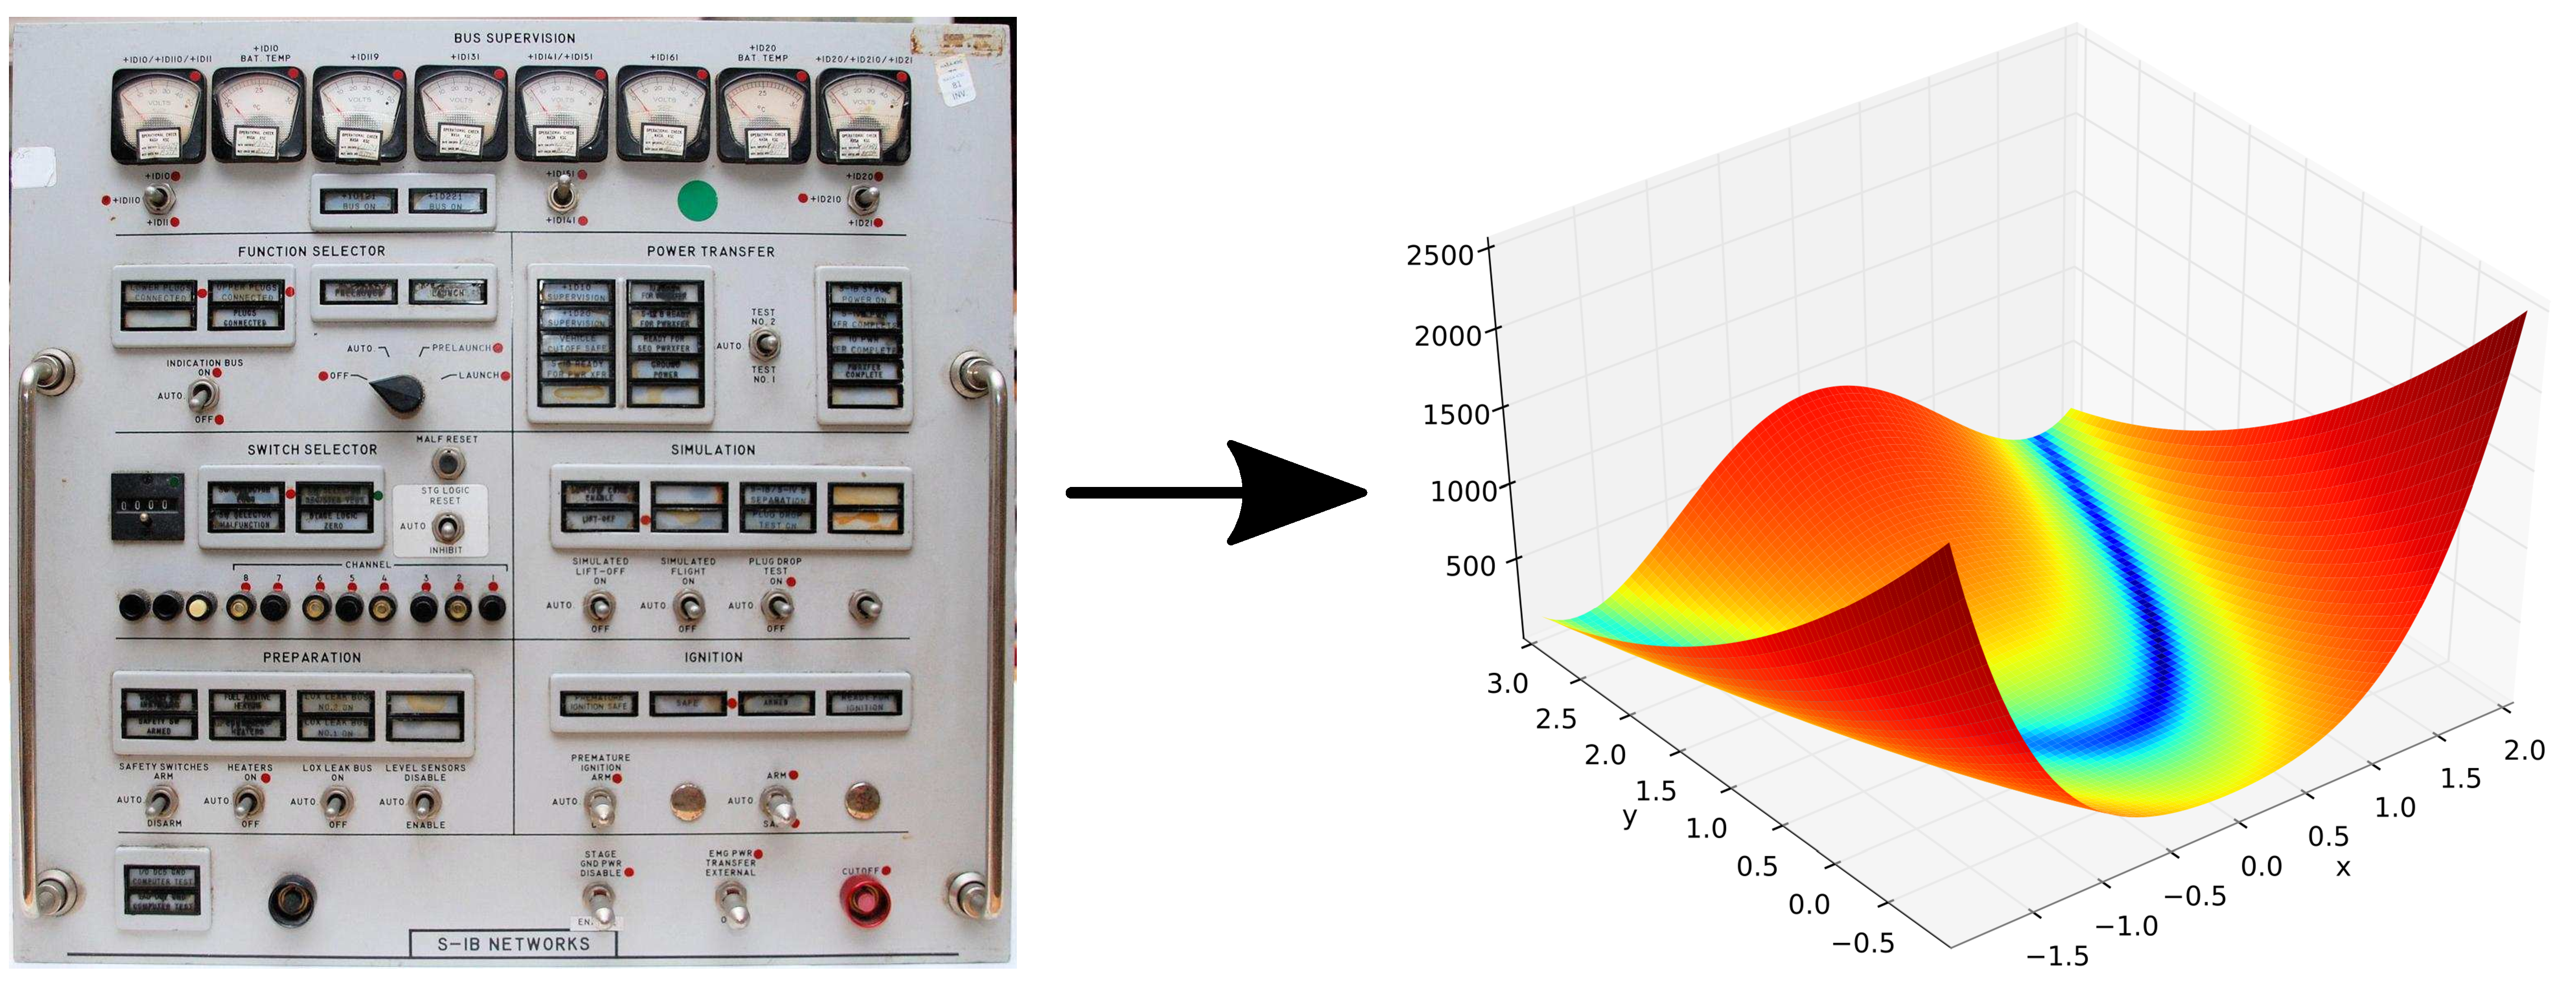
\includegraphics[width=1\textwidth]{autotuning}
  \end{figure}
\end{frame}

\begin{frame}[fragile]
  \frametitle{Autotuning: OpenTuner}
    \begin{columns}
        \column{0.5\textwidth}
        \begin{figure}[H]
            \centering
            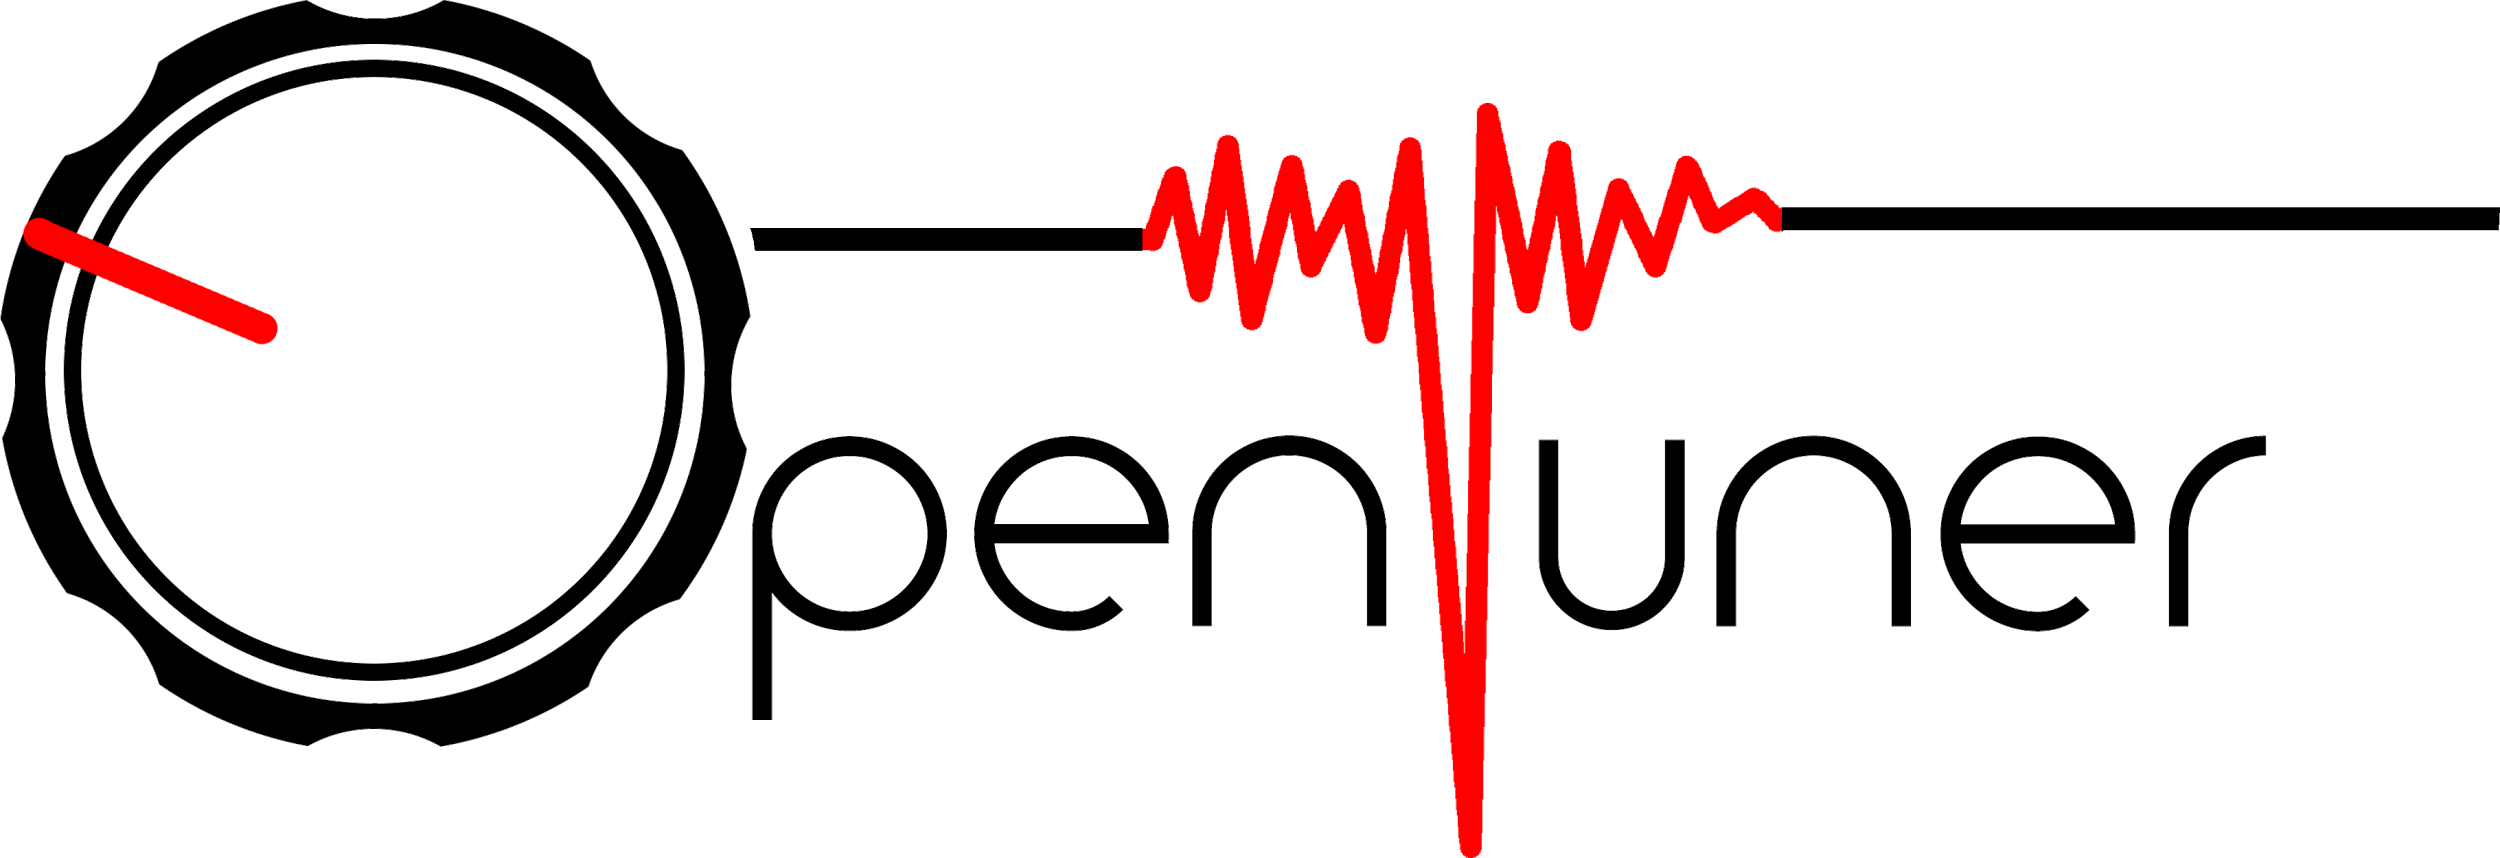
\includegraphics[width=0.55\textwidth]{opentuner-logo}
        \end{figure}%
        \begin{itemize}
            \item Autotuning framework
            \item Implements ensembles of search techniques
            \item Shares optimization results between techniques
        \end{itemize}
        \column{0.5\textwidth}
        \begin{figure}[H]
            \centering
            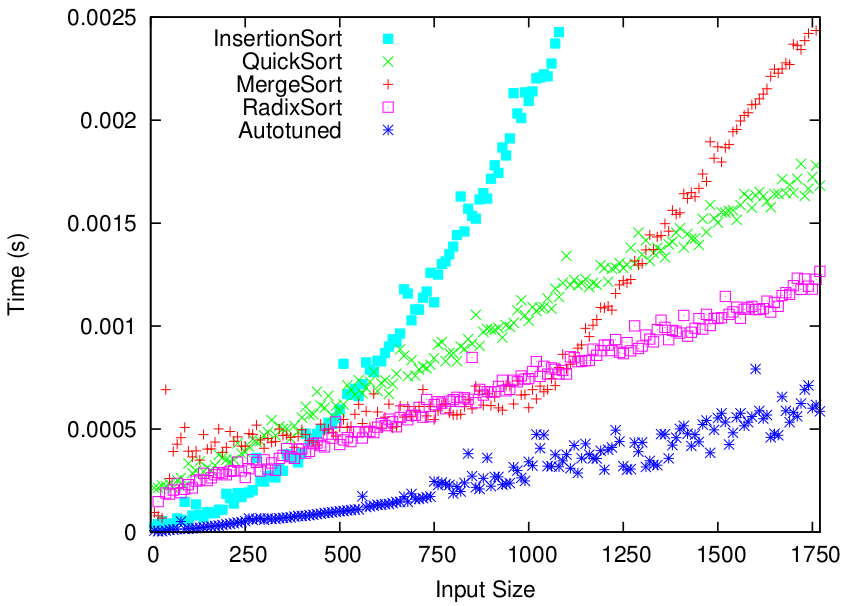
\includegraphics[width=1.05\textwidth]{sorting}
            \caption{Autotuning recursive sorting algorithms for an 8-core machine.}
        \end{figure}%
    \end{columns}
  \let\thefootnote\relax\footnotetext{Figure 1: Ansel, Jason, et al. "Opentuner: An extensible framework for program autotuning." Proceedings of the 23rd ICPAC. ACM, 2014.}
\end{frame}

\begin{frame}[fragile]
  \frametitle{Compiler Flags}
\newcolumntype{C}{>{\centering\arraybackslash}m{1.6cm}}
\newcolumntype{L}{>{\centering\arraybackslash}m{8cm}}
\newcolumntype{K}{>{\centering\arraybackslash}m{2cm}}
\newcolumntype{P}{>{\centering\arraybackslash}m{1.2cm}}
\begin{table}[htpb]
    \centering
    \footnotesize
        \begin{tabular}{@{}CL@{}}
        \toprule
        \textbf{Step} & \textbf{Options} \\ \midrule
        \textbf{NVCC} & \texttt{prec-sqrt}, \texttt{relocatable-device-code}, \texttt{no-align-double}, \texttt{use-fast-math}, \texttt{gpu-architecture}, \texttt{ftz}, \texttt{prec-div} \\ \midrule
        \textbf{PTX} &  \texttt{def-load-cache}, \texttt{opt-level}, \texttt{fmad}, \texttt{allow-expensive-optimizations}, \texttt{maxrregcount} \\ \midrule
        \textbf{NVLINK} & \texttt{preserve-relocs} \\ \bottomrule
    \end{tabular}%
    \\ \vspace{0.5cm}
    \begin{tabular}{@{}PKKKK@{}}
        \toprule
        \textbf{\scriptsize Options} & \texttt{\bf \scriptsize gpu-architecture} & \texttt{\bf \scriptsize opt-level} & \texttt{\bf \scriptsize def-load-cache} & \texttt{\bf \scriptsize maxrregcount} \\ \midrule
        \textbf{\scriptsize Values} & \texttt{\scriptsize sm\_20}, \texttt{\scriptsize sm\_21}, \texttt{\scriptsize sm\_30}, \texttt{\scriptsize sm\_32}, \texttt{\scriptsize sm\_35}  & \texttt{\scriptsize 0 - 1}  & \texttt{\scriptsize ca}, \texttt{\scriptsize cg}, \texttt{\scriptsize cv}, \texttt{\scriptsize cs} & \texttt{\scriptsize 16 - 64} \\ \bottomrule
    \end{tabular}
\end{table}
\end{frame}

\begin{frame}[fragile]
  \frametitle{GPU Testbed}
\newcommand{\specialcell}[2][c]{%
  \begin{tabular}[#1]{@{}c@{}}#2\end{tabular}}
  \centering
\begin{table}[thpb]
    \centering
    \scriptsize
    \begin{tabular}{cccccccc}
        \toprule
        \textbf{Model}&\textbf{c.c.}&\specialcell{\bf Global \\ \bf Memory}&\textbf{Bus}&\textbf{Bandwidth}&\textbf{L2}&\textbf{SM/Cores}&\textbf{Clock} \\ \midrule
        GTX-680&3.0&2 GB&256-bit&192.2 GB/s&512 KB&8/1536&1006 Mhz \\ \midrule
        Tesla-K20&3.5&4 GB&320-bit&208 GB/s&1280 KB&13/2496&706 Mhz \\ \midrule
        Tesla-K40&3.5&12 GB&384-bit&276.5 GB/s&1536 KB&15/2880&745 Mhz \\ \bottomrule
    \end{tabular}
\end{table}
\end{frame}

\begin{frame}[fragile]
    \frametitle{Experiments}
    All the results' data and the code for the experiments, the autotuner and
    the figures is hosted at \alert{\bf github.com/phrb/gpu-autotuning}, 
    under the GNU GPLv3 license.
\end{frame}

\begin{frame}[fragile]
    \frametitle{Experiments: Matrix Multiplication}
    Four optimizations of square matrix multiplication ($N = 1024$):
    \begin{itemize}
        \item \alert{\bf \#1}: Non-Coalesced accesses to Global Memory
        \item \alert{\bf \#2}: Coalesced accesses to Global Memory
        \item \alert{\bf \#3}: \alert{\bf\#1}, plus Shared Memory 
        \item \alert{\bf \#4}: \alert{\bf\#2}, plus Shared Memory
    \end{itemize}
\end{frame}

\begin{frame}[fragile]
    \frametitle{Experiments: Maximum Subarray}
    Find the maximum subsequence sum of an array ($N = 134217728$):
    \begin{itemize}
        \item \alert{\bf 4096} threads
        \item \alert{\bf 32} blocks of \alert{\bf 128} threads
    \end{itemize}
\end{frame}

\begin{frame}[fragile]
    \frametitle{Results: Optimization}
    \begin{figure}[htpb]
        \centering
        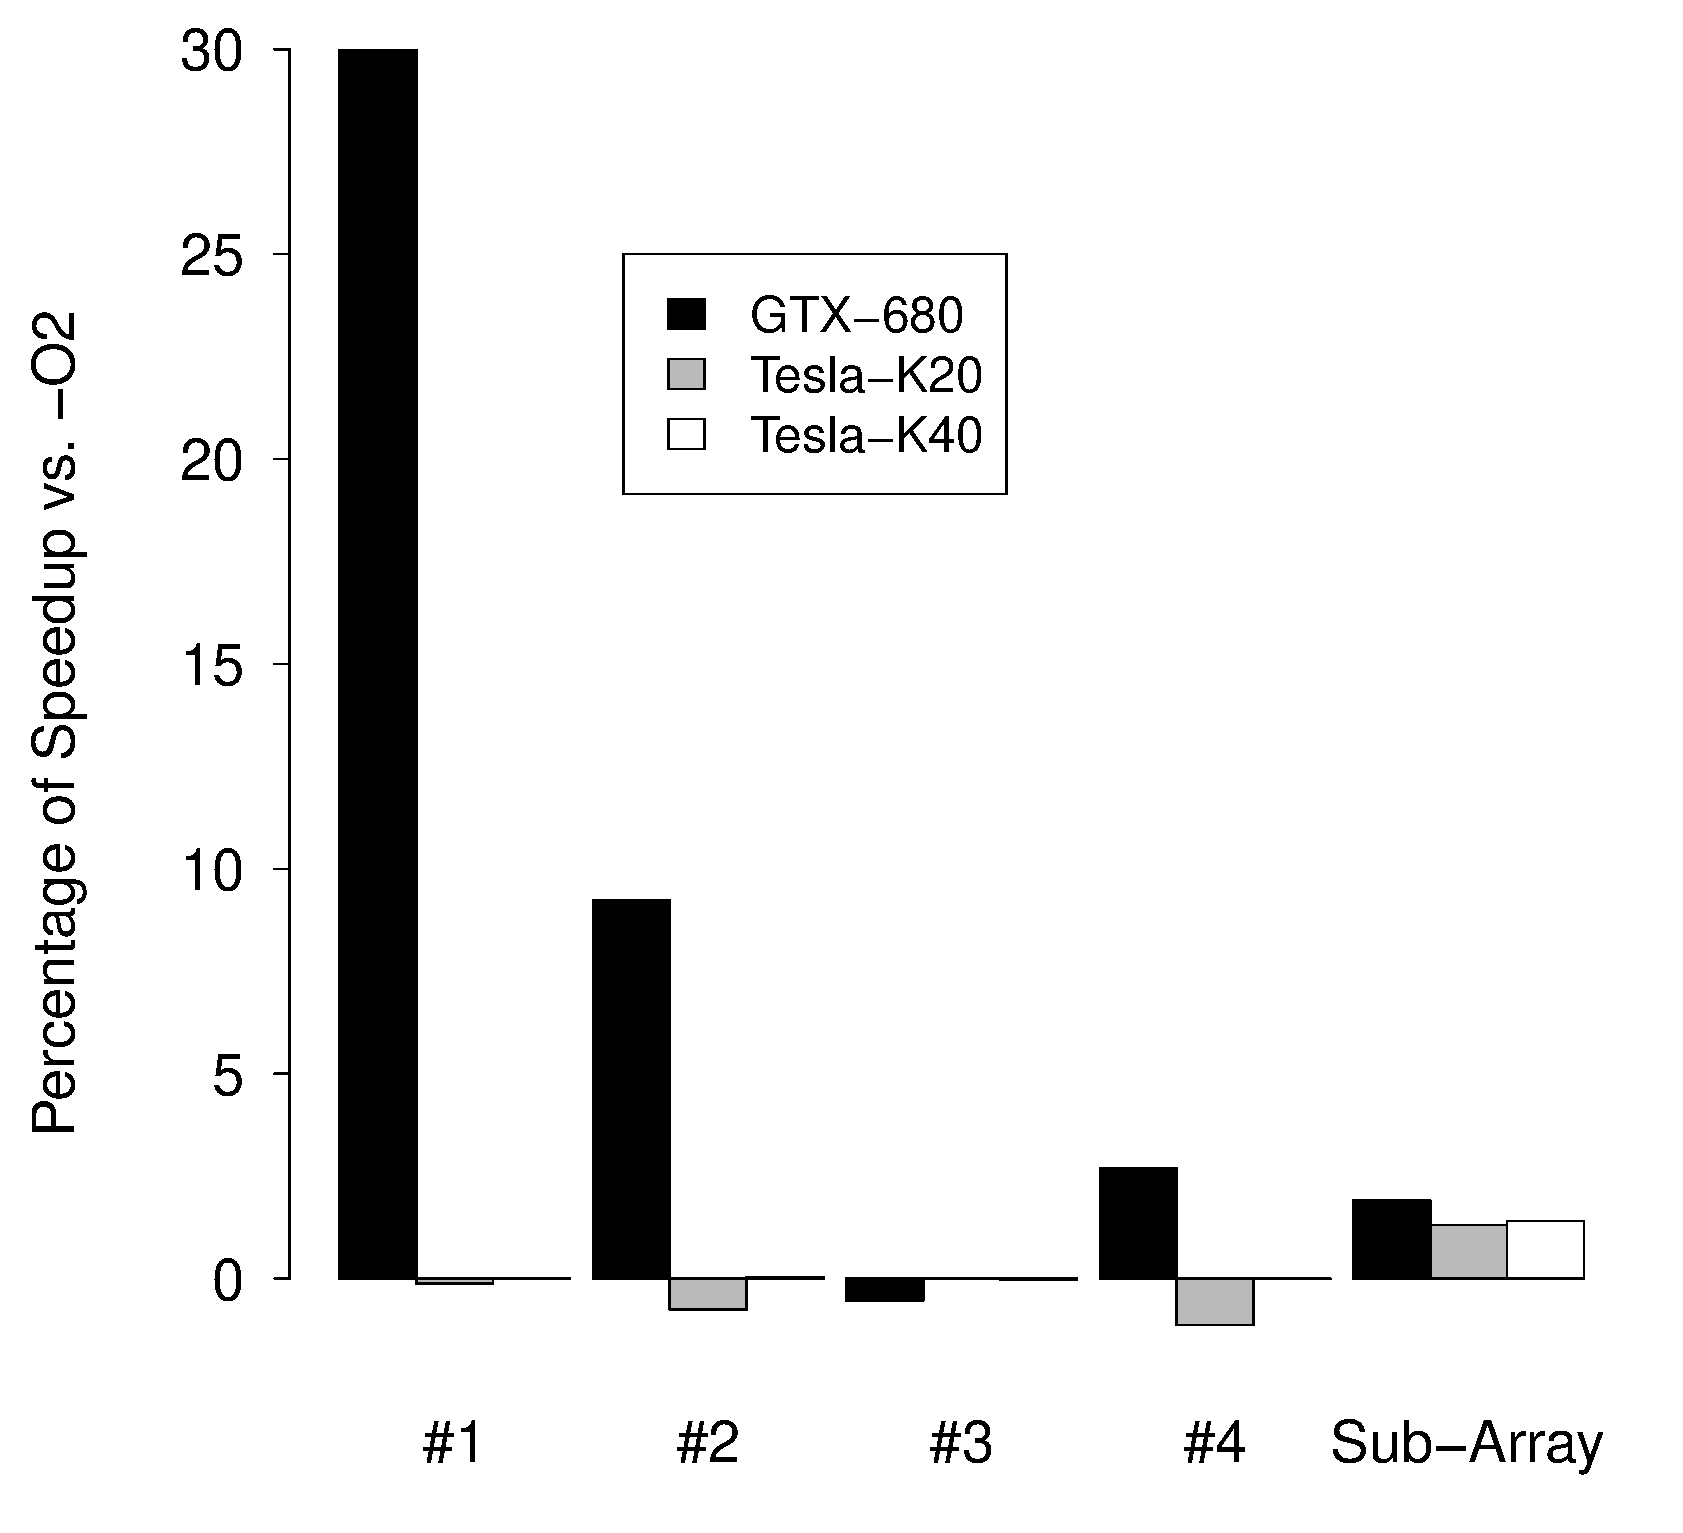
\includegraphics[width=0.8\textwidth]{Summary}
    \end{figure}
\end{frame}

\begin{frame}[fragile]
  \frametitle{Results: Optimization}
  Why did the \alert{\bf GTX-680} have the best results?

\newcommand{\specialcell}[2][c]{%
  \begin{tabular}[#1]{@{}c@{}}#2\end{tabular}}
  \centering
\begin{table}[thpb]
    \centering
    \scriptsize
    \begin{tabular}{cccccccc}
        \toprule
        \textbf{Model}&\textbf{c.c.}&\specialcell{\bf Global \\ \bf Memory}&\textbf{Bus}&\textbf{Bandwidth}&\textbf{L2}&\textbf{SM/Cores}&\textbf{Clock} \\ \midrule
        \alert{\bf GTX-680}&\alert{\bf 3.0}&\alert{\bf 2 GB}&\alert{\bf 256-bit}&\alert{\bf 192.2 GB/s}&\alert{\bf 512 KB}&\alert{\bf 8/1536}&\alert{\bf 1006 Mhz} \\ \midrule
        Tesla-K20&3.5&4 GB&320-bit&208 GB/s&1280 KB&13/2496&706 Mhz \\ \midrule
        Tesla-K40&3.5&12 GB&384-bit&276.5 GB/s&1536 KB&15/2880&745 Mhz \\ \bottomrule
    \end{tabular}
\end{table}
\end{frame}

\begin{frame}[fragile]
  \frametitle{Results: Autotuner}
  Results for optimization \alert{\bf \#2}
  in the \alert{\bf GTX-680}:

    \begin{figure}[htpb]
        \centering
        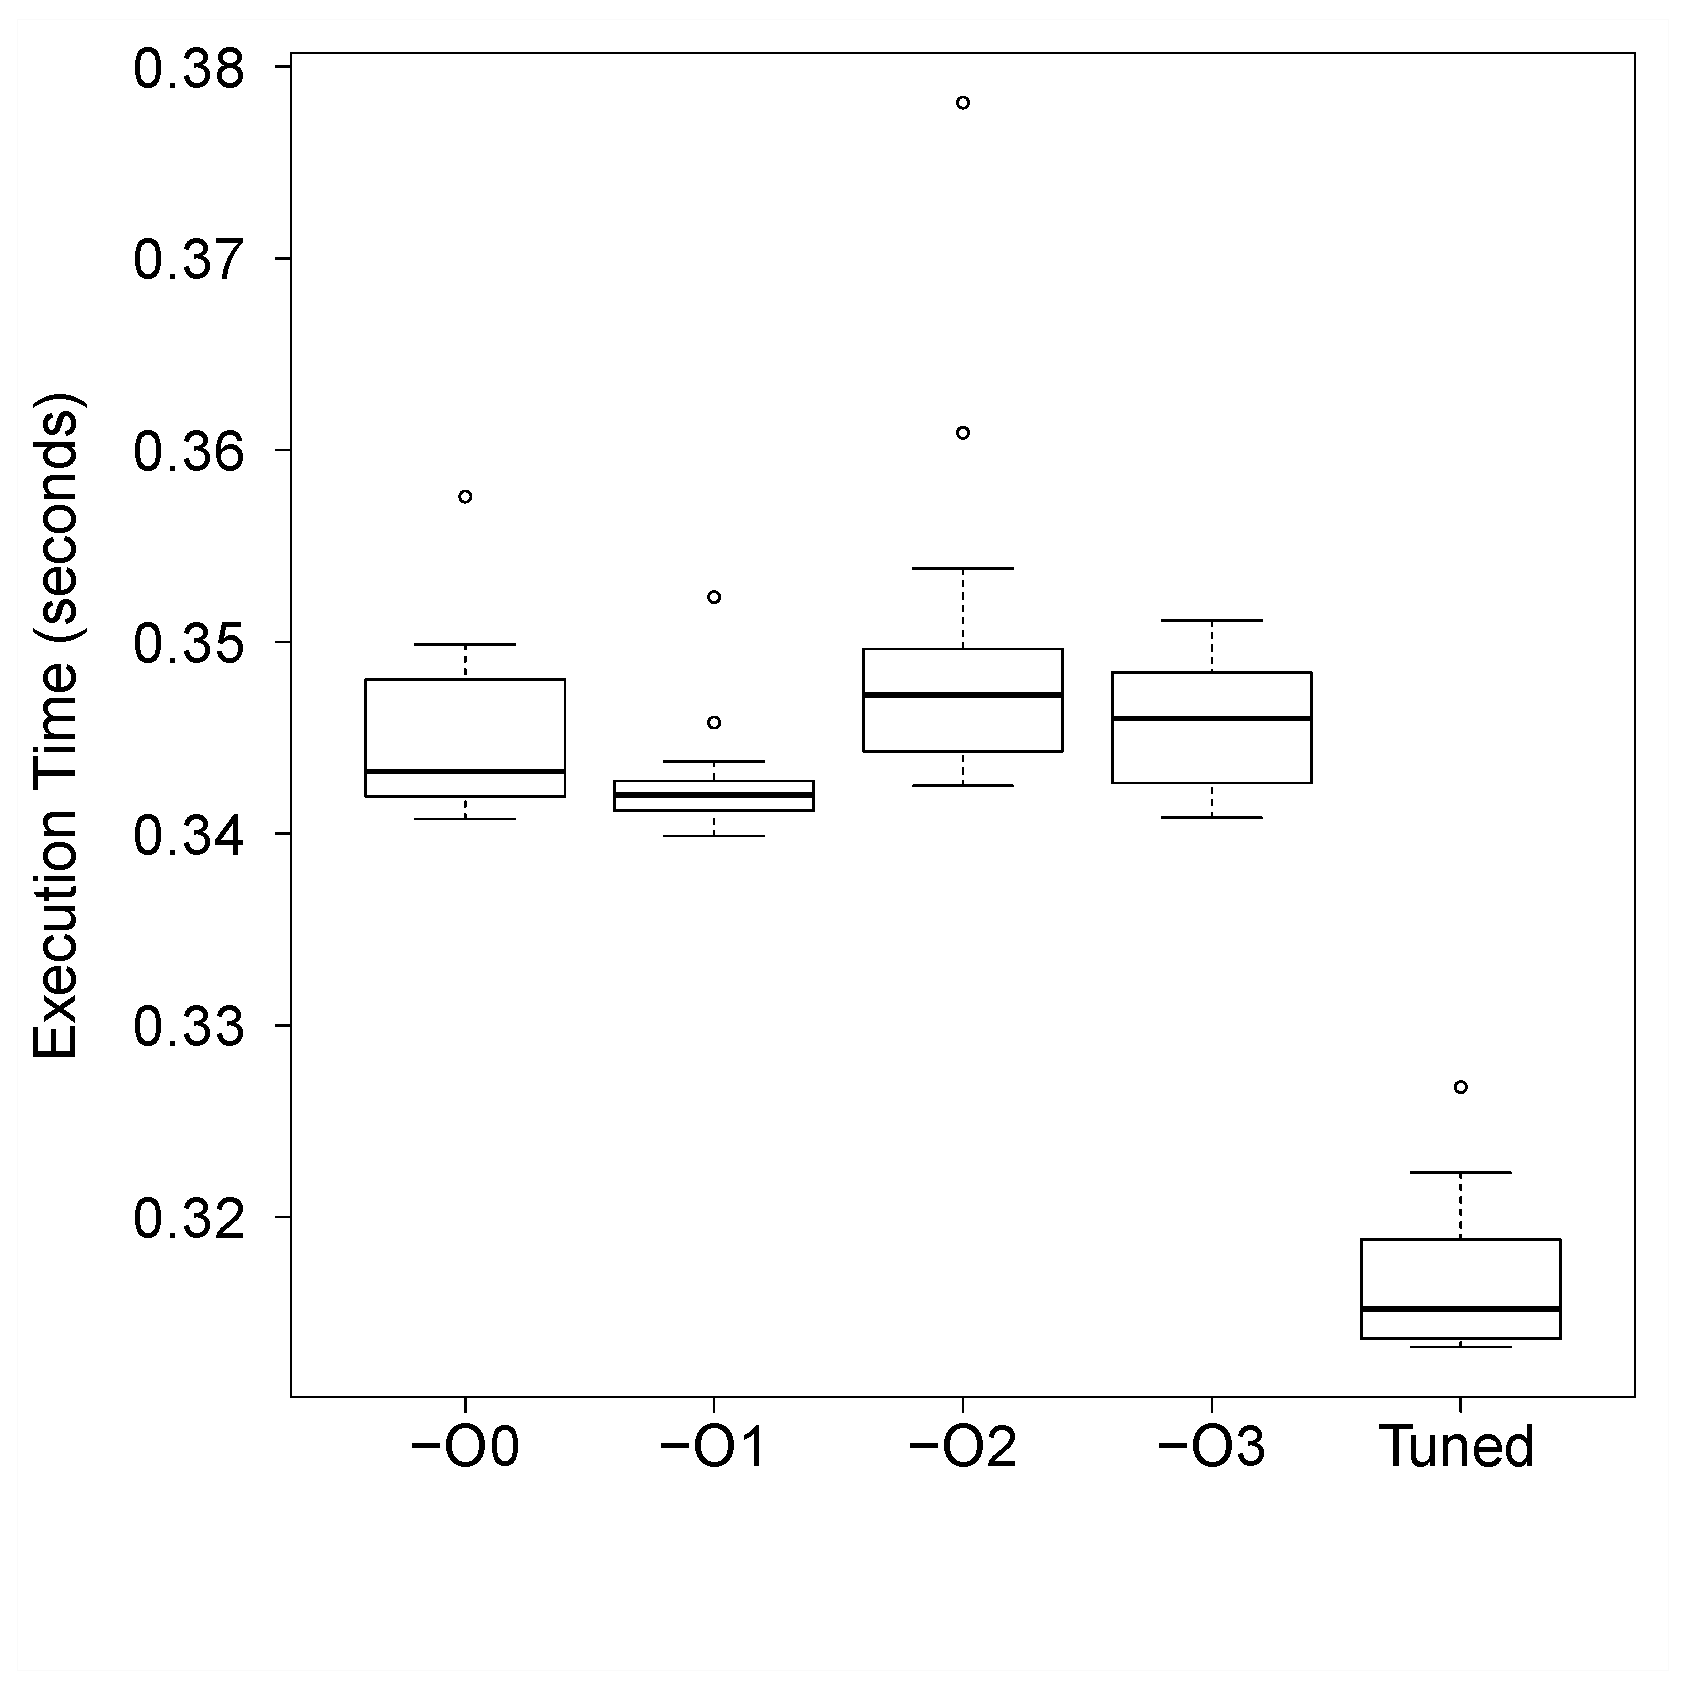
\includegraphics[width=0.75\textwidth]{MatMulGPU-GTX-680-Box.eps}
    \end{figure}
\end{frame}

\begin{frame}[fragile]
  \frametitle{Results: Autotuner}
  Results for optimization \alert{\bf \#2}
  in the \alert{\bf GTX-680}:

  \begin{figure}[htpb]
      \centering
      \begin{minipage}[t!]{.49\textwidth}
          \centering
          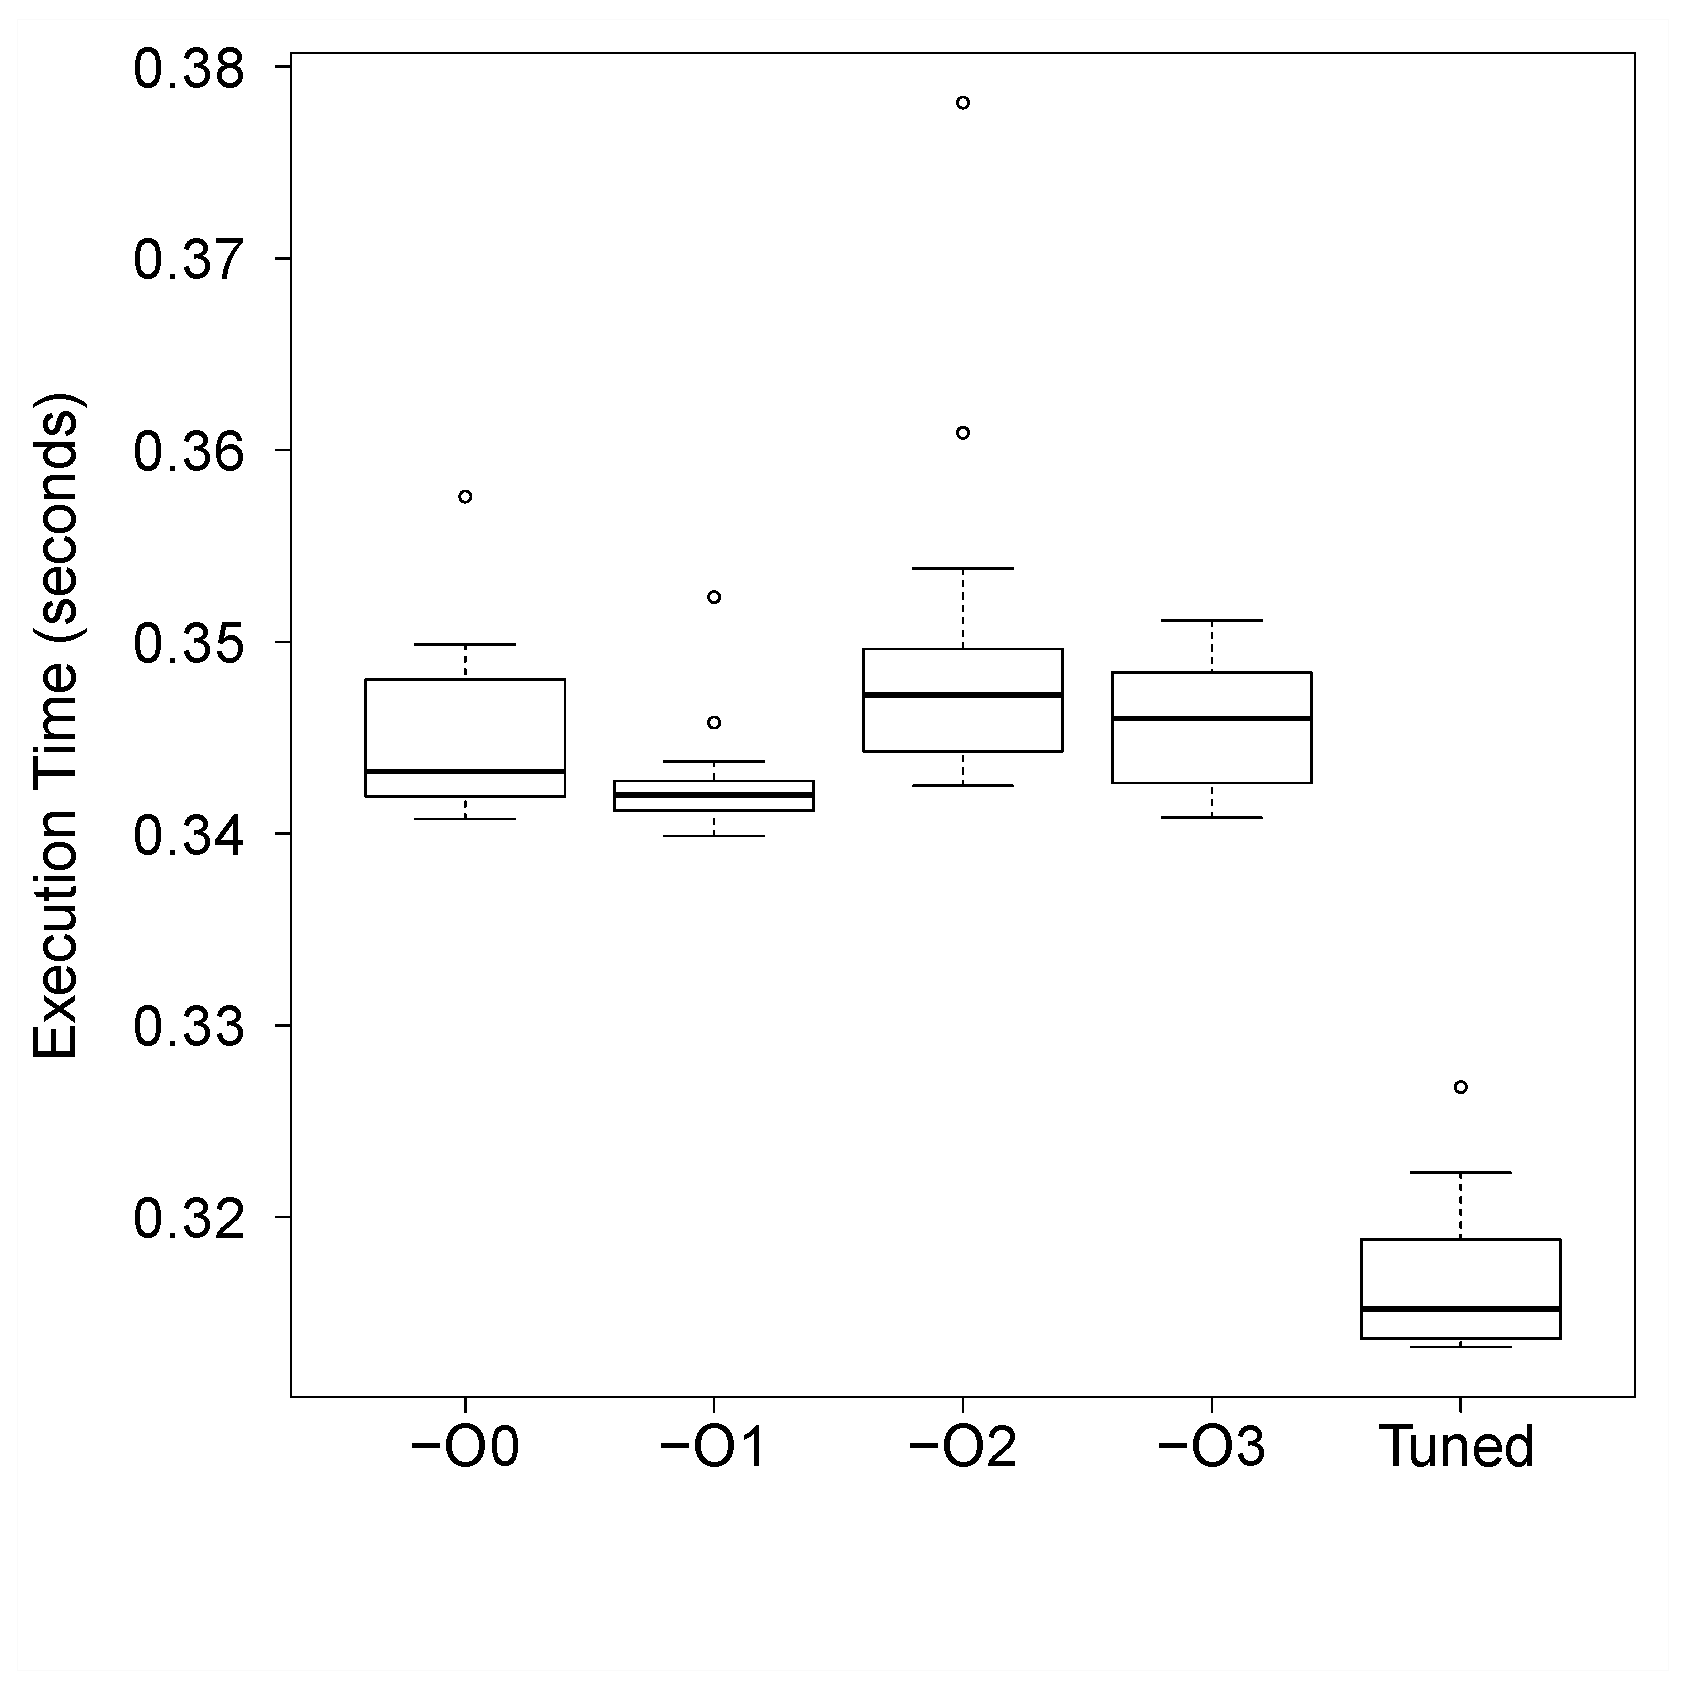
\includegraphics[width=\textwidth]{MatMulGPU-GTX-680-Box.eps}
      \end{minipage}%
      \hfill
      \begin{minipage}[t!]{.49\textwidth}
          \centering
          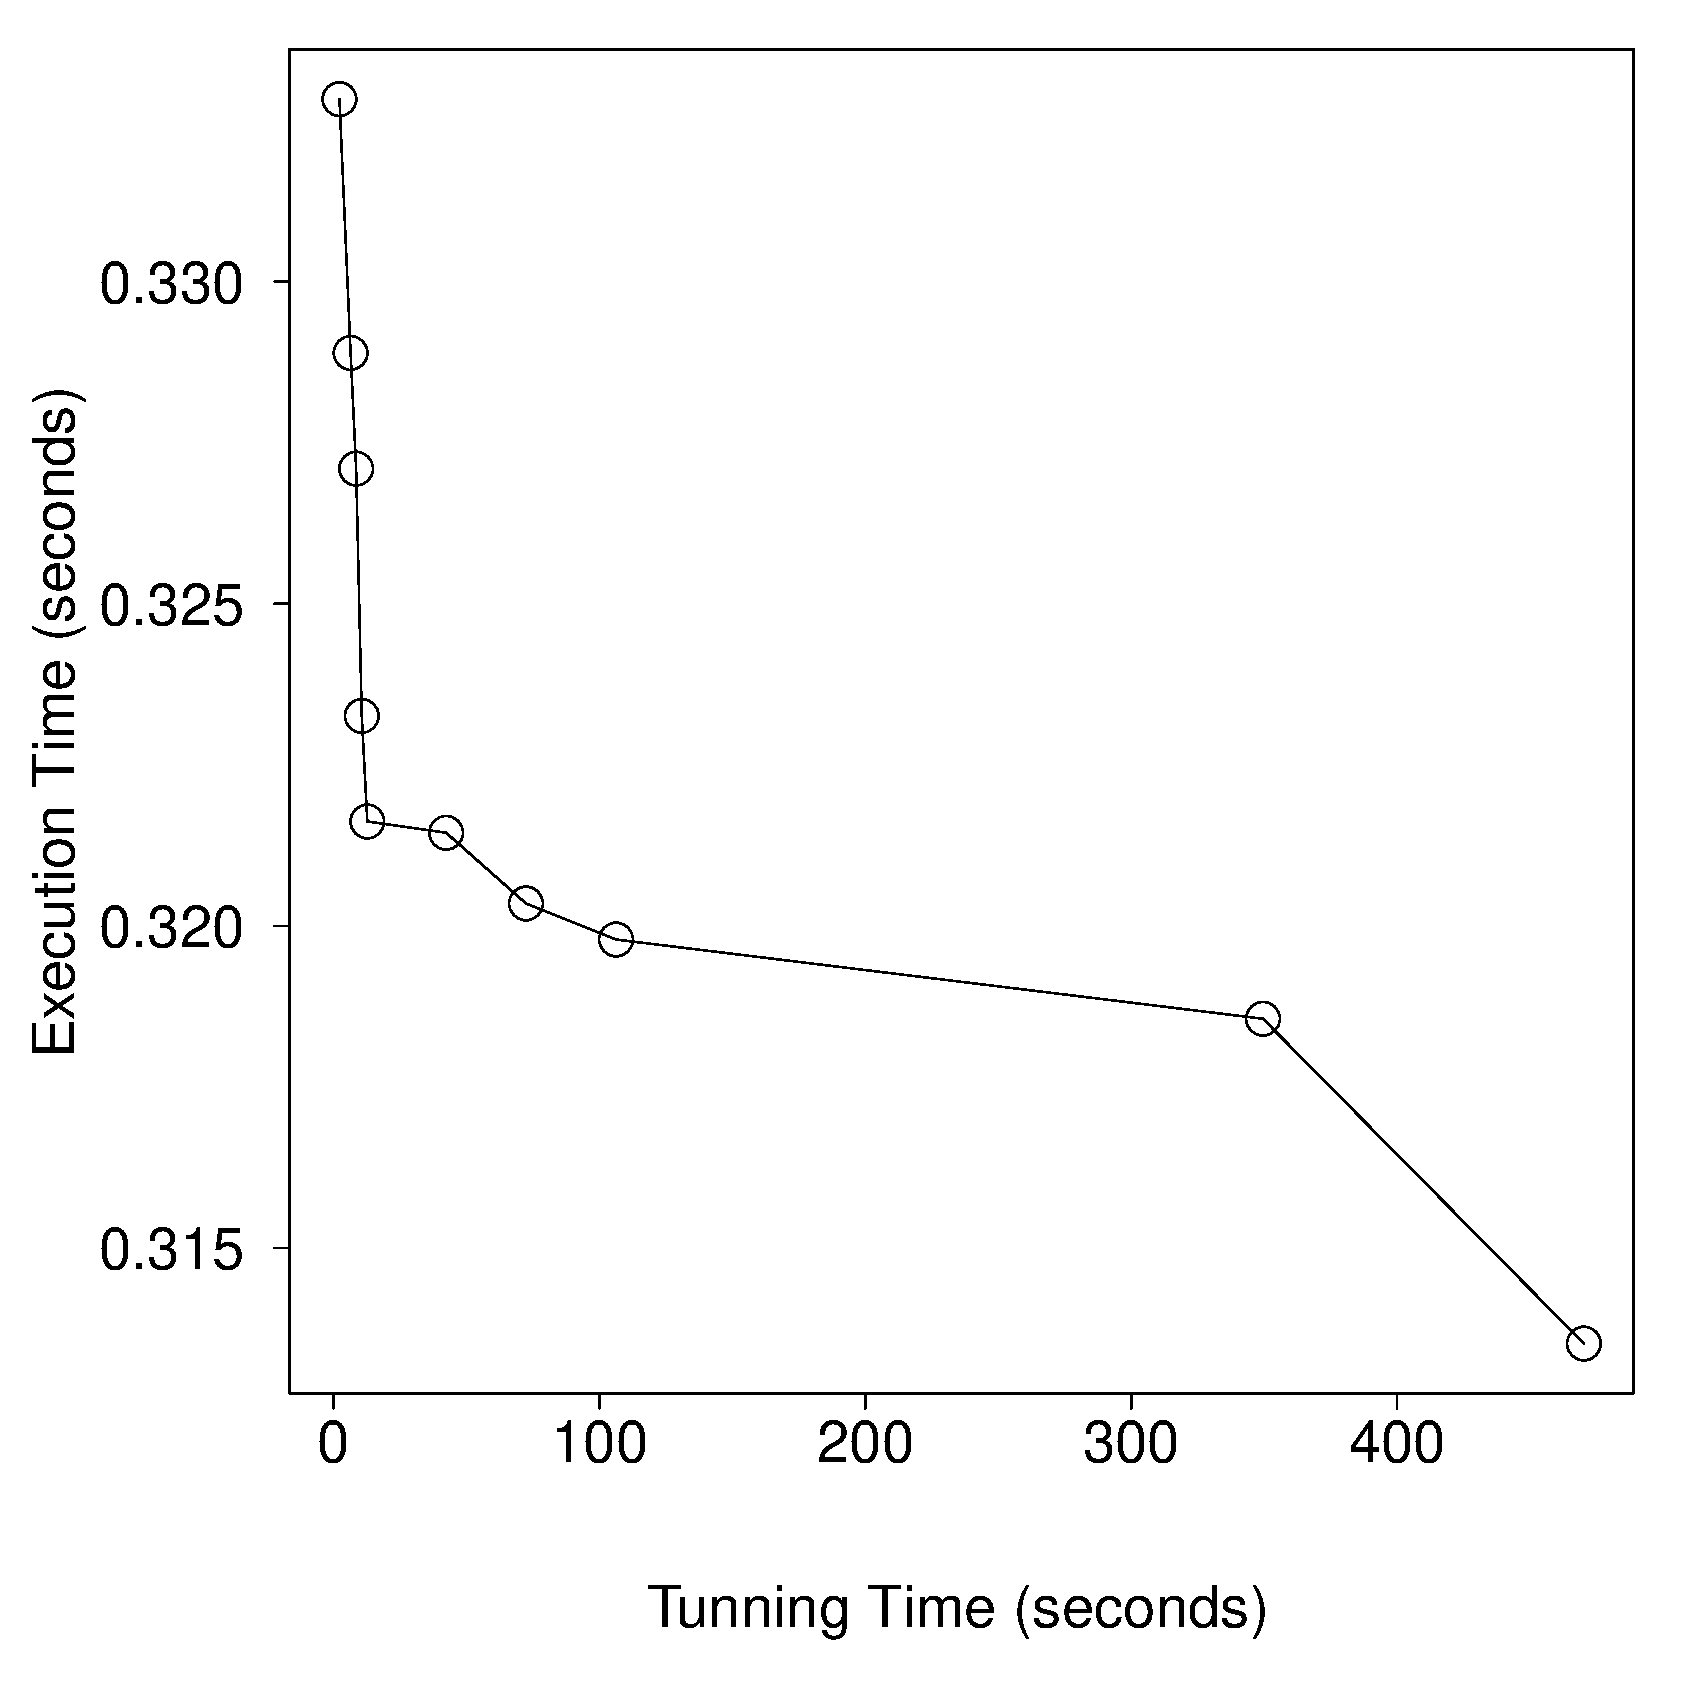
\includegraphics[width=\textwidth]{MatMulGPU-GTX-680-Best.eps}
      \end{minipage}%
  \end{figure}
\end{frame}

\begin{frame}[fragile]
    \frametitle{Results: Failed Configurations}
    \begin{figure}[htpb]
        \centering
        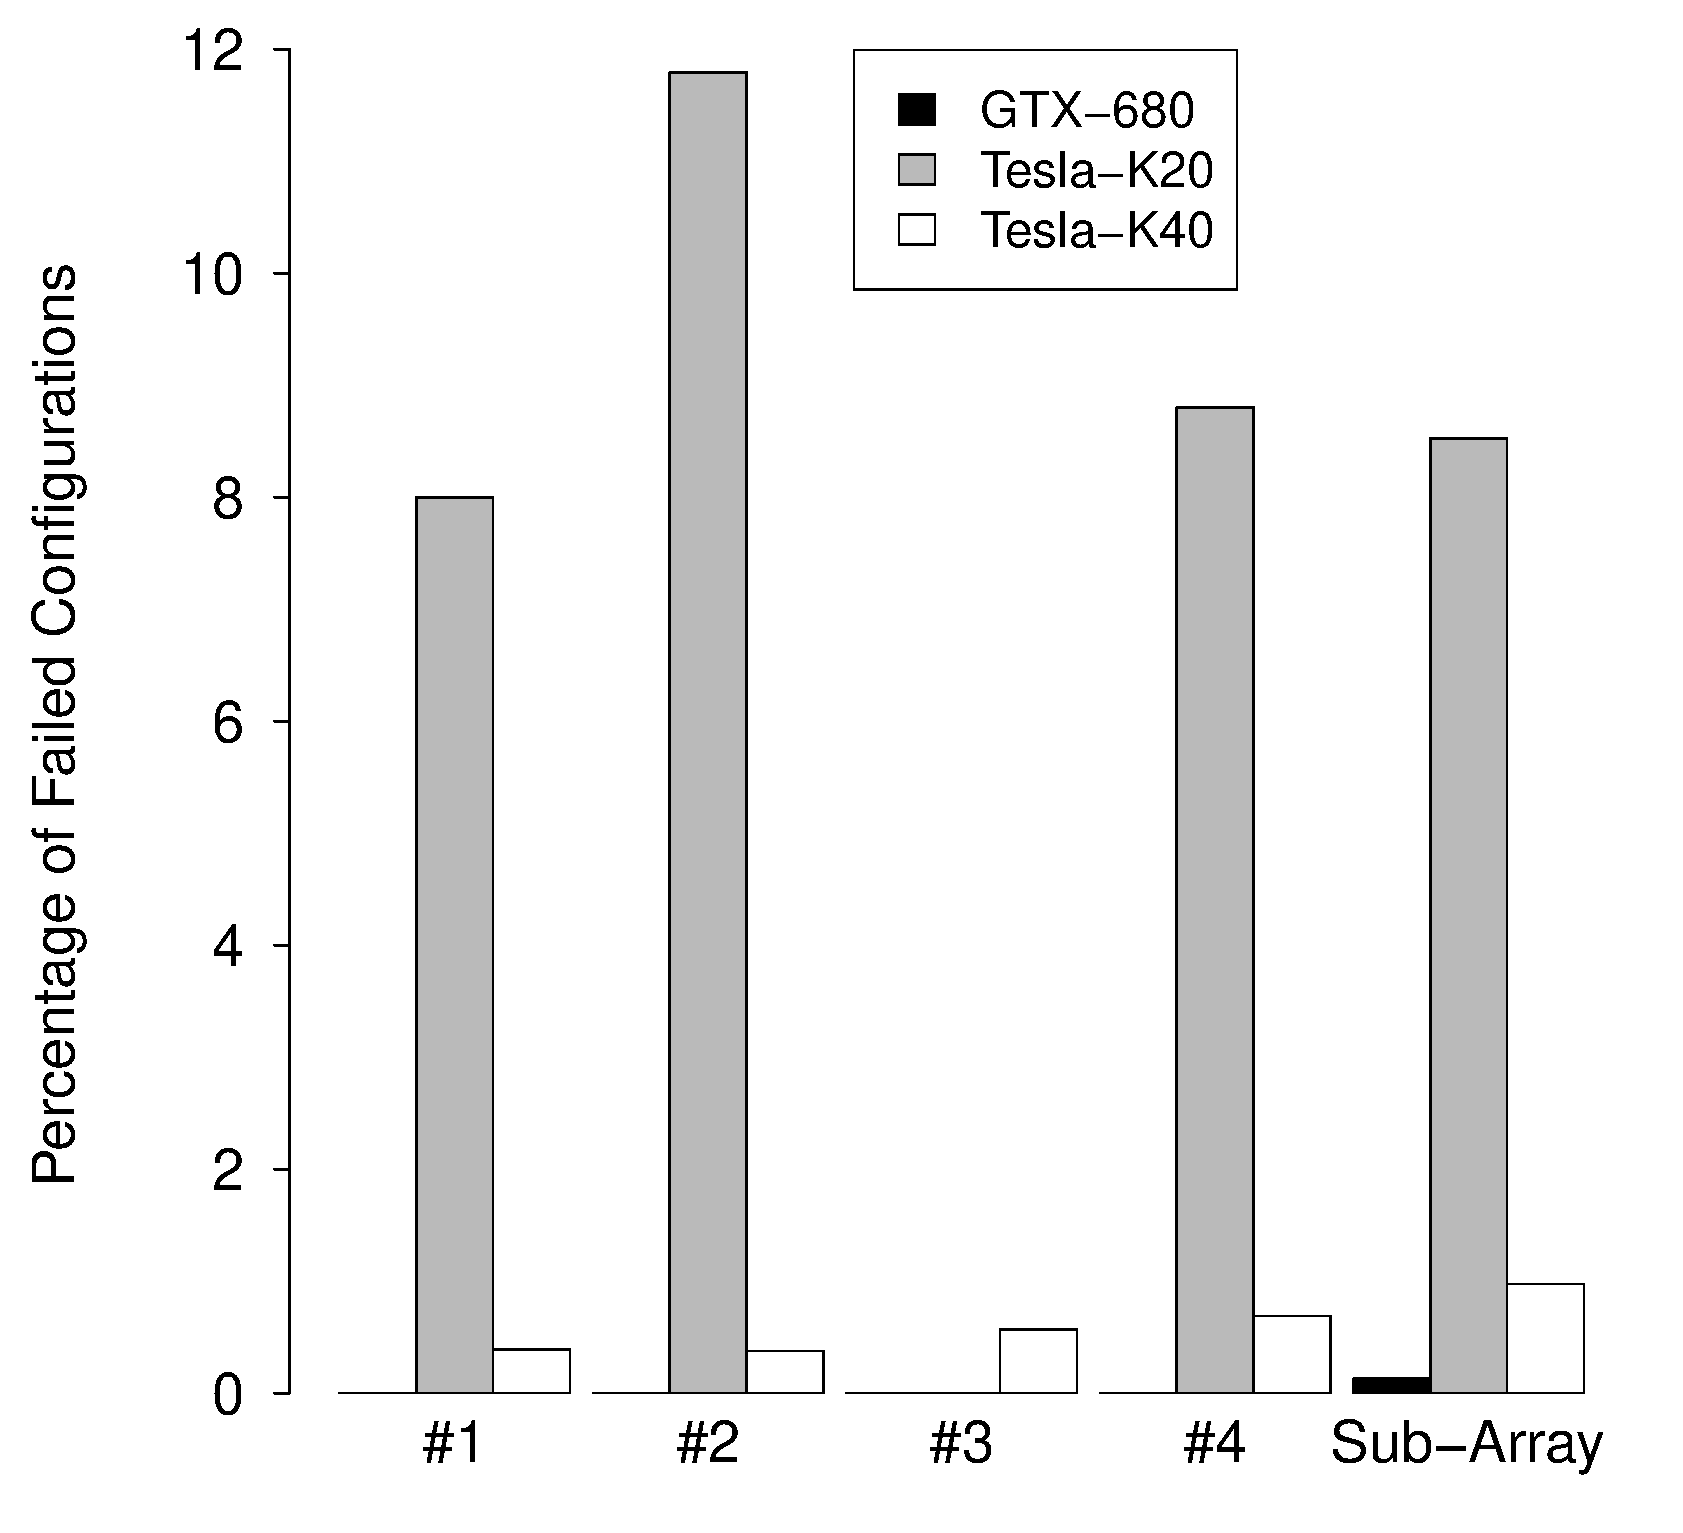
\includegraphics[width=0.8\textwidth]{FailedSummary}
    \end{figure}
\end{frame}

\begin{frame}[fragile]
  \frametitle{Results: Failed Configurations}
  Who's guilty?
  \begin{itemize}
      \item \alert{\bf sm\_32}, for \alert{\bf \#1} in the \alert{\bf K20} and \alert{\bf K40}
  \end{itemize}
\end{frame}

\begin{frame}[fragile]
  \frametitle{Conclusion}
  \begin{itemize}
      \item \alert{\bf 30\%} speedup for \alert{\bf \#1} in the \alert{\bf GTX-680}
          \pause
      \item \alert{\bf Different} parameters for each GPU
          \pause
      \item \alert{\bf Always} assert the results
  \end{itemize}
\end{frame}

\plain{Thank you!}

\maketitle

\end{document}
